%%%%%%%%%%%%%%%%%%%%% chapter.tex %%%%%%%%%%%%%%%%%%%%%%%%%%%%%%%%%
%
% sample chapter
%
% Use this file as a template for your own input.
%
%%%%%%%%%%%%%%%%%%%%%%%% Springer-Verlag %%%%%%%%%%%%%%%%%%%%%%%%%%
%\motto{Use the template \emph{chapter.tex} to style the various elements of your chapter content.}

\chapter{Rosetta Code Tasks starting with P}

\section*{Palindrome detection}

Write at least one function/method (or whatever it is called in your
preferred language) to check if a sequence of characters (or bytes) is a
\href{http://en.wikipedia.org/wiki/Palindrome}{palindrome} or not. The
\emph{function} must return a boolean value (or something that can be
used as boolean value, like an integer).

It is not mandatory to write also an example code that uses the
\emph{function}, unless its usage could be not clear (e.g. the provided
recursive C solution needs explanation on how to call the function).

It is not mandatory to handle properly encodings (see
\emph{String length}), i.e. it is admissible that
the function does not recognize `salàlas' as palindrome.

The function must not ignore spaces and punctuations. The compliance to
the aforementioned, strict or not, requirements completes the task.

\textbf{Example}\\ An example of a Latin palindrome is the sentence
"\emph{In girum imus nocte et consumimur igni}", roughly translated as:
we walk around in the night and we are burnt by the fire (of love). To
do your test with it, you must make it all the same case and strip
spaces.

\textbf{Notes}\\

\begin{itemize}
\item
  It might be useful for this task to know how to
  \emph{reverse a string}.
\item
  This task's entries might also form the subjects of the task
  \emph{Test a function}.
\end{itemize}


\begin{wideverbatim}

(de palindrome? (S)
   (= (setq S (chop S)) (reverse S)) )

Output:

: (palindrome? "ingirumimusnocteetconsumimurigni")
-> T

\end{wideverbatim}

\pagebreak{}
\section*{Pangram checker}

Write a function or method to check a sentence to see if it is a
\href{http://en.wikipedia.org/wiki/Pangram}{pangram} or not and show its
use.

A pangram is a sentence that contains all the letters of the English
alphabet at least once, for example: \emph{The quick brown fox jumps
over the lazy dog}.

\begin{wideverbatim}

(de isPangram (Str)
   (not
      (diff
         '`(chop "abcdefghijklmnopqrstuvwxyz")
         (chop (lowc Str)) ) ) )

\end{wideverbatim}

\pagebreak{}
\section*{Parallel calculations}

Many programming languages allow you to specify computations to be run
in parallel. While \emph{Concurrent
computing} is focused on concurrency, the purpose of this task is to
distribute time-consuming calculations on as many CPUs as possible.

Assume we have a collection of numbers, and want to find the one with
the largest minimal prime factor (that is, the one that contains
relatively large factors). To speed up the search, the factorization
should be done in parallel using separate threads or processes, to take
advantage of multi-core CPUs.

Show how this can be formulated in your language. Parallelize the
factorization of those numbers, then search the returned list of numbers
and factors for the largest minimal factor, and return that number and
its prime factors.

For the prime number decomposition you may use the solution of the
\emph{Prime decomposition} task.


The prime decomposition of a number is defined as a list of prime
numbers which when all multiplied together, are equal to that number.
Example: 12 = 2 × 2 × 3, so its prime decomposition is \{2, 2, 3\}

Write a function which returns an \emph{array} or
\emph{collection} which contains the prime
decomposition of a given number, n, greater than 1. If your language
does not have an isPrime-like function available, you may assume that
you have a function which determines whether a number is prime (note its
name before your code).

If you would like to test code from this task, you may use code from
\emph{trial division} or the
\emph{Sieve of Eratosthenes}.

Note: The program must not be limited by the word size of your computer
or some other artificial limit; it should work for any number regardless
of size (ignoring the physical limits of RAM etc).


\begin{wideverbatim}

The '[http://software-lab.de/doc/refL.html#later later]' function is used in
PicoLisp to start parallel computations. The following solution calls 'later' on


Create a program to continually calculate and output the next digit of π
(pi). The program should continue forever (until it is aborted by the
user) calculating and outputting each digit in succession. The output
should be a decimal sequence beginning 3.14159265 \ldots{}


the 'factor' function from [[Prime decomposition#PicoLisp]], and then
'[http://software-lab.de/doc/refW.html#wait wait]'s until all results are
available:

(let Lst
   (mapcan
      '((N)
         (later (cons)               # When done,
            (cons N (factor N)) ) )  # return the number and its factors
      (quote
         188573867500151328137405845301  # Process a collection of 12 numbers
         3326500147448018653351160281
         979950537738920439376739947
         2297143294659738998811251
         136725986940237175592672413
         3922278474227311428906119
         839038954347805828784081
         42834604813424961061749793
         2651919914968647665159621
         967022047408233232418982157
         2532817738450130259664889
         122811709478644363796375689 ) )
   (wait NIL (full Lst))  # Wait until all computations are done
   (maxi '((L) (apply min L)) Lst) )  # Result: Number in CAR, factors in CDR

Output:

-> (2532817738450130259664889 6531761 146889539 2639871491)

\end{wideverbatim}

\pagebreak{}
\section*{Parametric polymorphism}

Create two classes Point(x,y) and Circle(x,y,r) with a polymorphic
function print, accessors for (x,y,r), copy constructor, assignment and
destructor and every possible default constructors

\href{http://en.wikipedia.org/wiki/Parametric\_Polymorphism}{Parametric
Polymorphism} is a way to define types or functions that are generic
over other types. The genericity can be expressed by using \emph{type
variables} for the parameter type, and by a mechanism to explicitly or
implicitly replace the type variables with concrete types when
necessary.

Write a small example for a type declaration that is parametric over
another type, together with a short bit of code (and its type signature)
that uses it. A good example is a container type, let's say a binary
tree, together with some function that traverses the tree, say, a
\emph{map}-function that operates on every element of the tree.

This language feature only applies to statically-typed languages.

\begin{wideverbatim}

PicoLisp is dynamically-typed, so in principle every function is polymetric over
its arguments. It is up to the function to decide what to do with them. A
function traversing a tree, modifying the nodes in-place (no matter what the
type of the node is):

(de mapTree (Tree Fun)
   (set Tree (Fun (car Tree)))
   (and (cadr Tree) (mapTree @ Fun))
   (and (cddr Tree) (mapTree @ Fun)) )

Test:

(balance 'MyTree (range 1 7))          # Create a tree of numbers
-> NIL

: (view MyTree T)                      # Display it
      7
   6
      5
4
      3
   2
      1
-> NIL


: (mapTree MyTree inc)                 # Increment all nodes
-> NIL

: (view MyTree T)                      # Display the tree
      8
   7
      6
5
      4
   3
      2
-> NIL

\end{wideverbatim}

\begin{wideverbatim}

: (balance 'MyTree '("a" "b" "c" "d" "e" "f" "g"))  # Create a tree of strings
-> NIL

: (view MyTree T)                      # Display it
      "g"
   "f"
      "e"
"d"
      "c"
   "b"
      "a"
-> NIL

: (mapTree MyTree uppc)                # Convert all nodes to upper case
-> NIL

: (view MyTree T)                      # Display the tree
      "G"
   "F"
      "E"
"D"
      "C"
   "B"
      "A"
-> NIL

\end{wideverbatim}

\pagebreak{}
\section*{Parametrized SQL statement}

Parameterized SQL statements are an easy way to avoid
\href{http://en.wikipedia.org/wiki/SQL\_injection}{SQL injection}
attacks. SQL drivers and libraries will automatically ``sanitize'' input
to parameterized SQL statements to avoid these catastrophic database
attacks.

Using a SQL update statement like this one (spacing is optional):


\begin{wideverbatim}
UPDATE players
   SET name = 'Smith, Steve', score = 42, active = TRUE
   WHERE jerseyNum = 99
\end{wideverbatim}

show how to make a parameterized SQL statement, set the parameters to
the values given above, and execute the statement.

\begin{wideverbatim}

As PicoLisp uses normal function calls for DB manipulations, parameters are
always treated as plain data and are not executed.

(for P (collect 'jerseyNum '+Players 99)
   (put!> P 'name "Smith, Steve")
   (put!> P 'score 42)
   (put!> P 'active T) )

\end{wideverbatim}

\pagebreak{}
\section*{Parse an IP Address}

The purpose of this task is to demonstrate parsing of text-format IP
addresses, using IPv4 and IPv6.

Taking the following as inputs:

\ctable[pos = H, center, botcap]{ll}
{% notes
}
{% rows
\FL
127.0.0.1 & The ``localhost'' IPv4 address
\\\noalign{\medskip}
127.0.0.1:80 & The ``localhost'' IPv4 address, with a specified port
(80)
\\\noalign{\medskip}
::1 & The ``localhost'' IPv6 address
\\\noalign{\medskip}
{[}::1{]}:80 & The ``localhost'' IPv6 address, with a specified port
(80)
\\\noalign{\medskip}
2605:2700:0:3::4713:93e3 & Rosetta Code's primary server's public IPv6
address
\\\noalign{\medskip}
{[}2605:2700:0:3::4713:93e3{]}:80 & Rosetta Code's primary server's
public IPv6 address, with a specified port (80)
\LL
}

Emit each described IP address as a hexadecimal integer representing the
address, the address space, and the port number specified, if any. In
languages where variant result types are clumsy, the result should be
ipv4 or ipv6 address number, something which says which address space
was represented, port number and something that says if the port was
specified.

For example 127.0.0.1 has the address number 7F000001 (2130706433
decimal) in the ipv4 address space. ~::ffff:127.0.0.1 represents the
same address in the ipv6 address space where it has the address number
FFFF7F000001 (281472812449793 decimal). Meanwhile~::1 has address number
1 and serves the same purpose in the ipv6 address space that 127.0.0.1
serves in the ipv4 address space.

\begin{wideverbatim}

# Return a cons pair of address and port: (address . port)
(de ipAddress (Adr)
   (use (@A @B @C @D @Port)
      (cond
         ((match '("[" @A "]" ":" @Port) Adr)
            (adrIPv6 (split @A ":") @Port) )
         ((match '("[" @A "]") Adr)
            (adrIPv6 (split @A ":")) )
         ((match '(@A ":" @B ":" @C) Adr)
            (adrIPv6 (cons @A @B (split @C ":"))) )
         ((match '(@A "." @B "." @C "." @D ":" @Port) Adr)
            (adrIPv4 (list @A @B @C @D) @Port) )
         ((match '(@A "." @B "." @C "." @D) Adr)
            (adrIPv4 (list @A @B @C @D)) )
         (T (quit "Bad IP address" (pack Adr))) ) ) )

(de adrIPv4 (Lst Port)
   (cons
      (sum >> (-24 -16 -8 0) (mapcar format Lst))
      (format Port) ) )

(de adrIPv6 (Lst Port)
   (cons
      (sum >>
         (-112 -96 -80 -64 -48 -32 -16 0)
         (mapcan
            '((X)
               (if X
                  (cons (hex X))
                  (need (- 9 (length Lst)) 0) ) )  # Handle '::'
            (cons (or (car Lst) "0") (cdr Lst)) ) )
      (format Port) ) )

\end{wideverbatim}

\begin{wideverbatim}

Test:

(for A
   (quote
      "127.0.0.1"
      "127.0.0.1:80"
      "::1"
      "[::1]:80"
      "2605:2700:0:3::4713:93e3"
      "[2605:2700:0:3::4713:93e3]:80" )
   (let I (ipAddress (chop A))
      (tab (-29 34 40 7)
         A
         (hex (car I))
         (format (car I))
         (cdr I) ) ) )

Output:

127.0.0.1        7F000001   2130706433
127.0.0.1:80     7F000001   2130706433     80
::1              1          1
[::1]:80         1          1              80
2605:2700:0:3::4713:93e3       260527000000000300000000471393E3  
50537416338094019778974086937420469219
[2605:2700:0:3::4713:93e3]:80  260527000000000300000000471393E3  
50537416338094019778974086937420469219     80

\end{wideverbatim}

\pagebreak{}
\section*{Parsing command-line arguments}

\emph{Command-line arguments} can be quite complicated, as in ``nc -v
-n -z -w 1 192.168.1.2 1-1000''. Many languages provide a library
(getopt or GetOpt) to parse the raw command line options in an
intelligent way.

\begin{wideverbatim}

PicoLisp doesn't have a library to get options. Instead, the command line is
parsed at startup and handled in the following way: Each command line argument
is executed (interpreted) as a Lisp source file, except that if the first
character is a hypen '-', then that arguments is taken as a Lisp function call
(without the surrounding parentheses). For example, the command line

\$ ./pil abc.l -foo def.l -"bar 3 4" -'mumble "hello"' -bye

has the effect that

# The file "abc.l" is executed
# (foo) is called
# The file "def.l" is executed
# (bar 3 4) is called
# (mumble "hello") is called
# (bye) is called, resulting in program termination

Command line arguments like "-v", "-n" and "-z" can be implemented simply by
defining three functions 'v', 'n' and 'z'.

In addition to the above mechanism, the command line can also be handled
"manually", by either processing the list of arguments returned by
'[http://software-lab.de/doc/refA.html#argv argv]', or by fetching arguments
individually with '[http://software-lab.de/doc/refO.html#opt opt]'.

\end{wideverbatim}

\pagebreak{}
\section*{Parsing/RPN calculator algorithm}

Create a stack-based evaluator for an expression in
\href{http://en.wikipedia.org/wiki/Reverse\_Polish\_notation}{reverse
Polish notation} that also shows the changes in the stack as each
individual token is processed \emph{as a table}.

\begin{itemize}
\item
  Assume an input of a correct, space separated, string of tokens of an
  RPN expression
\item Test with the RPN expression generated from the
  \emph{Parsing/Shunting-yard algorithm} task \texttt{'3 4 2 * 1 5 - 2
    3 \^{} \^{} / +'} then print and display the output here.
\end{itemize}

\begin{description}
\item[Note]
\end{description}

\begin{itemize}
\item
  `\^{}' means exponentiation in the expression above.
\end{itemize}

\begin{description}
\item[See also]
\end{description}

\begin{itemize}
\item \emph{Parsing/Shunting-yard algorithm} for a method of
  generating an RPN from an infix expression.
\item
  Several solutions to \emph{24 game/Solve} make
  use of RPN evaluators (although tracing how they work is not a part of
  that task).
\item \emph{Parsing/RPN to infix conversion}.
\item
  \emph{Arithmetic evaluation}.
\end{itemize}


\begin{wideverbatim}

This is an integer-only calculator:

(de rpnCalculator (Str)
   (let (^ **  Stack)  # Define '^' from the built-in '**'
      (prinl "Token  Stack")
      (for Token (str Str "*+-/\^")
         (if (num? Token)
            (push 'Stack @)
            (set (cdr Stack)
               (Token (cadr Stack) (pop 'Stack)) ) )
         (prin Token)
         (space 6)
         (println Stack) )
      (println (car Stack)) ) )

Test (note that the top-of-stack is in the left-most position):

: (rpnCalculator "3 4 2 * 1 5 - 2 3 \^ \^ / +")
Token  Stack
3      (3)
4      (4 3)
2      (2 4 3)
*      (8 3)
1      (1 8 3)
5      (5 1 8 3)
-      (-4 8 3)
2      (2 -4 8 3)
3      (3 2 -4 8 3)
^      (8 -4 8 3)
^      (65536 8 3)
/      (0 3)
+      (3)
3
-> 3

\end{wideverbatim}

\pagebreak{}
\section*{Parsing/RPN to infix conversion}

Create a program that takes an
\href{http://en.wikipedia.org/wiki/Reverse\_Polish\_notation}{RPN}
representation of an expression formatted as a space separated sequence
of tokens and generates the equivalent expression in
\href{http://en.wikipedia.org/wiki/Infix\_notation}{infix notation}.

\begin{itemize}
\item
  Assume an input of a correct, space separated, string of tokens
\item
  Generate a space separated output string representing the same
  expression in infix notation
\item
  Show how the major datastructure of your algorithm changes with each
  new token parsed.
\item
  Test with the following input RPN strings then print and display the
  output here.
\end{itemize}

\ctable[pos = H, center, botcap]{ll}
{% notes
}
{% rows
\FL
RPN input & sample output
\ML
\texttt{3 4 2 * 1 5 - 2 3 \^{} \^{} / +} & \texttt{3 + 4 * 2 / ( 1 - 5 ) \^{} 2 \^{} 3}
\\\noalign{\medskip}
\texttt{1 2 + 3 4 + \^{} 5 6 + \^{}} & \texttt{( ( 1 + 2 ) \^{} ( 3 + 4 ) ) \^{} ( 5 + 6 )}
\LL
}

\begin{itemize}
\item
  Operator precedence is given in this table:
\end{itemize}

\ctable[pos = H, center, botcap]{lll}
{% notes
}
{% rows
\FL
operator & \href{http://en.wikipedia.org/wiki/Order\_of\_operations}{precedence} & \href{http://en.wikipedia.org/wiki/Operator\_associativity}{associativity}
\ML
\^{} & 4 & Right
\\\noalign{\medskip}
* & 3 & Left
\\\noalign{\medskip}
/ & 3 & Left
\\\noalign{\medskip}
+ & 2 & Left
\\\noalign{\medskip}
- & 2 & Left
\LL
}

\begin{description}
\item[Note]  `\^{}' means exponentiation.
\end{description}

\begin{description}
\item[See also]
\end{description}

\begin{itemize}
\item
  \emph{Parsing/Shunting-yard
  algorithm} for a method of generating an RPN from an infix expression.
\item
  \emph{Parsing/RPN calculator
  algorithm} for a method of calculating a final value from this output
  RPN expression.
\item
  \href{http://www.rubyquiz.com/quiz148.html}{Postfix to infix} from the
  RubyQuiz site.
\end{itemize}


\begin{wideverbatim}

We maintain a stack of cons pairs, consisting of precedences and partial
expressions. Numbers get a "highest" precedence of '9'.

(de leftAssoc (Op)
   (member Op '("*" "/" "+" "-")) )

(de precedence (Op)
   (case Op
      ("\^" 4)
      (("*" "/") 3)
      (("+" "-") 2) ) )

(de rpnToInfix (Str)
   (let Stack NIL
      (prinl "Token  Stack")
      (for Token (str Str "_")
         (cond
            ((num? Token) (push 'Stack (cons 9 @)))  # Highest precedence
            ((not (cdr Stack)) (quit "Stack empty"))
            (T
               (let (X (pop 'Stack)  P (precedence Token))
                  (set Stack
                     (cons P
                        (pack
                           (if ((if (leftAssoc Token) < <=) (caar Stack) P)
                              (pack "(" (cdar Stack) ")")
                              (cdar Stack) )
                           " " Token " "
                           (if ((if (leftAssoc Token) <= <) (car X) P)
                              (pack "(" (cdr X) ")")
                              (cdr X) ) ) ) ) ) ) )
         (prin Token)
         (space 6)
         (println Stack) )
      (prog1 (cdr (pop 'Stack))
         (and Stack (quit "Garbage remained on stack")) ) ) )

\end{wideverbatim}

\begin{wideverbatim}

Test (note that the top-of-stack is in the left-most position):

: (rpnToInfix "3 4 2 * 1 5 - 2 3 \^ \^ / +")
Token  Stack
3      ((9 . 3))
4      ((9 . 4) (9 . 3))
2      ((9 . 2) (9 . 4) (9 . 3))
*      ((3 . "4 * 2") (9 . 3))
1      ((9 . 1) (3 . "4 * 2") (9 . 3))
5      ((9 . 5) (9 . 1) (3 . "4 * 2") (9 . 3))
-      ((2 . "1 - 5") (3 . "4 * 2") (9 . 3))
2      ((9 . 2) (2 . "1 - 5") (3 . "4 * 2") (9 . 3))
3      ((9 . 3) (9 . 2) (2 . "1 - 5") (3 . "4 * 2") (9 . 3))
^      ((4 . "2 \^ 3") (2 . "1 - 5") (3 . "4 * 2") (9 . 3))
^      ((4 . "(1 - 5) \^ 2 \^ 3") (3 . "4 * 2") (9 . 3))
/      ((3 . "4 * 2 / (1 - 5) \^ 2 \^ 3") (9 . 3))
+      ((2 . "3 + 4 * 2 / (1 - 5) \^ 2 \^ 3"))
-> "3 + 4 * 2 / (1 - 5) \^ 2 \^ 3"

: (rpnToInfix "1 2 + 3 4 + \^ 5 6 + \^")
Token  Stack
1      ((9 . 1))
2      ((9 . 2) (9 . 1))
+      ((2 . "1 + 2"))
3      ((9 . 3) (2 . "1 + 2"))
4      ((9 . 4) (9 . 3) (2 . "1 + 2"))
+      ((2 . "3 + 4") (2 . "1 + 2"))
^      ((4 . "(1 + 2) \^ (3 + 4)"))
5      ((9 . 5) (4 . "(1 + 2) \^ (3 + 4)"))
6      ((9 . 6) (9 . 5) (4 . "(1 + 2) \^ (3 + 4)"))
+      ((2 . "5 + 6") (4 . "(1 + 2) \^ (3 + 4)"))
^      ((4 . "((1 + 2) \^ (3 + 4)) \^ (5 + 6)"))
-> "((1 + 2) \^ (3 + 4)) \^ (5 + 6)"

\end{wideverbatim}

\pagebreak{}
\section*{Parsing/Shunting-yard algorithm}

Given the operator characteristics and input from the
\href{http://en.wikipedia.org/wiki/Shunting-yard\_algorithm}{Shunting-yard
algorithm} page and tables Use the algorithm to show the changes in the
operator stack and RPN output as each individual token is processed.

\begin{itemize}
\item
  Assume an input of a correct, space separated, string of tokens
  representing an infix expression
\item
  Generate a space separated output string representing the RPN
\item
  Test with the input string
  \texttt{'3 + 4 * 2 / ( 1 - 5 ) \^{} 2 \^{} 3'} then print and display
  the output here.
\item
  Operator precedence is given in this table:
\end{itemize}

\ctable[pos = H, center, botcap]{lll}
{% notes
}
{% rows
\FL
operator & precedence & associativity
\ML
\^{} & 4 & Right
\\\noalign{\medskip}
* & 3 & Left
\\\noalign{\medskip}
/ & 3 & Left
\\\noalign{\medskip}
+ & 2 & Left
\\\noalign{\medskip}
- & 2 & Left
\LL
}

\begin{description}
\item[Extra credit]
\end{description}

\begin{itemize}
\item
  Add extra text explaining the actions and an optional comment for the
  action on receipt of each token.
\end{itemize}

\begin{description}
\item[Note]
\end{description}

\begin{itemize}
\item
  the handling of functions and arguments is not required.
\end{itemize}

\begin{description}
\item[See also]
\end{description}

\begin{itemize}
\item \emph{Parsing/RPN calculator algorithm} for a method of
  calculating a final value from this output RPN expression.
\item \emph{Parsing/RPN to infix conversion}.
\end{itemize}


\begin{wideverbatim}

Note: "^" is a meta-character and must be escaped in strings

(de operator (Op)
   (member Op '("\^" "*" "/" "+" "-")) )

(de leftAssoc (Op)
   (member Op '("*" "/" "+" "-")) )

(de precedence (Op)
   (case Op
      ("\^" 4)
      (("*" "/") 3)
      (("+" "-") 2) ) )

(de shuntingYard (Str)
   (make
      (let (Fmt (-7 -30 -4)  Stack)
         (tab Fmt "Token" "Output" "Stack")
         (for Token (str Str "_")
            (cond
               ((num? Token) (link @))
               ((= "(" Token) (push 'Stack Token))
               ((= ")" Token)
                  (until (= "(" (car Stack))
                     (unless Stack
                        (quit "Unbalanced Stack") )
                     (link (pop 'Stack)) )
                  (pop 'Stack) )
               (T
                  (while
                     (and
                        (operator (car Stack))
                        ((if (leftAssoc (car Stack)) <= <)
                           (precedence Token)
                           (precedence (car Stack)) ) )
                     (link (pop 'Stack)) )
                  (push 'Stack Token) ) )
            (tab Fmt Token (glue " " (made)) Stack) )
         (while Stack
            (when (= "(" (car Stack))
               (quit "Unbalanced Stack") )
            (link (pop 'Stack))
            (tab Fmt NIL (glue " " (made)) Stack) ) ) ) )

\end{wideverbatim}

\begin{wideverbatim}

Output:

: (shuntingYard "3 + 4 * 2 / (1 - 5) \^ 2 \^ 3")
Token  Output                        Stack
3      3
+      3                             +
4      3 4                           +
*      3 4                           *+
2      3 4 2                         *+
/      3 4 2 *                       /+
(      3 4 2 *                       (/+
1      3 4 2 * 1                     (/+
-      3 4 2 * 1                     -(/+
5      3 4 2 * 1 5                   -(/+
)      3 4 2 * 1 5 -                 /+
^      3 4 2 * 1 5 -                 ^/+
2      3 4 2 * 1 5 - 2               ^/+
^      3 4 2 * 1 5 - 2               ^^/+
3      3 4 2 * 1 5 - 2 3             ^^/+
       3 4 2 * 1 5 - 2 3 ^           ^/+
       3 4 2 * 1 5 - 2 3 ^ ^         /+
       3 4 2 * 1 5 - 2 3 ^ ^ /       +
       3 4 2 * 1 5 - 2 3 ^ ^ / +
-> (3 4 2 "*" 1 5 "-" 2 3 "\^" "\^" "/" "+")

\end{wideverbatim}

\pagebreak{}
\section*{Partial function application}

\href{http://en.wikipedia.org/wiki/Partial\_application}{Partial
function application} is the ability to take a function of many
parameters and apply arguments to some of the parameters to create a new
function that needs only the application of the remaining arguments to
produce the equivalent of applying all arguments to the original
function.

E.g:

Given values \texttt{v1, v2}

Given \texttt{f(param1, param2)}

Then \texttt{partial(f, param1=v1)} returns \texttt{f'(param2)}

And \texttt{f(param1=v1, param2=v2) == f'(param2=v2)} (for any value v2)

Note that in the partial application of a parameter, (in the above case
param1), other parameters are not explicitly mentioned. This is a
recurring feature of partial function application.

Task

\begin{itemize}
\item
  Create a function fs( f, s ) that takes a function, f( n ), of one
  value and a sequence of values s.\\ Function fs should return an
  ordered sequence of the result of applying function f to every value
  of s in turn.
\end{itemize}

\begin{itemize}
\item
  Create function f1 that takes a value and returns it multiplied by 2.
\item
  Create function f2 that takes a value and returns it squared.
\end{itemize}

\begin{itemize}
\item
  Partially apply f1 to fs to form function fsf1( s )
\item
  Partially apply f2 to fs to form function fsf2( s )
\end{itemize}

\begin{itemize}
\item
  Test fsf1 and fsf2 by evaluating them with s being the sequence of
  integers from 0 to 3 inclusive and then the sequence of even integers
  from 2 to 8 inclusive.
\end{itemize}

Notes

\begin{itemize}
\item
  In partially applying the functions f1 or f2 to fs, there should be no
  \emph{explicit} mention of any other parameters to fs, although
  introspection of fs within the partial applicator to find its
  parameters \emph{is} allowed.
\item
  This task is more about \emph{how} results are generated rather than
  just getting results.
\end{itemize}


\begin{wideverbatim}

(def 'fs mapcar)
(de f1 (N) (* 2 N))
(de f2 (N) (* N N))

(de partial (F1 F2)
   (curry (F1 F2) @
      (pass F1 F2) ) )

(def 'fsf1 (partial fs f1))
(def 'fsf2 (partial fs f2))

(for S '((0 1 2 3) (2 4 6 8))
   (println (fsf1 S))
   (println (fsf2 S)) )

Output:

(0 2 4 6)
(0 1 4 9)
(4 8 12 16)
(4 16 36 64)

\end{wideverbatim}

\pagebreak{}
\section*{Pascal's triangle}


Pascal's triangle is an interesting math concept. Its first few rows
look like this:

\begin{wideverbatim}
   1
  1 1
 1 2 1
1 3 3 1
\end{wideverbatim}

where each element of each row is either 1 or the sum of the two
elements right above it. For example, the next row would be 1 (since the
first element of each row doesn't have two elements above it), 4 (1 +
3), 6 (3 + 3), 4 (3 + 1), and 1 (since the last element of each row
doesn't have two elements above it). Each row \texttt{n} (starting with
row 0 at the top) shows the coefficients of the binomial expansion of (x
+ y)\textsuperscript{n}.

Write a function that prints out the first n rows of the triangle (with
\texttt{f(1)} yielding the row consisting of only the element 1). This
can be done either by summing elements from the previous rows or using a
binary coefficient or combination function. Behavior for
\texttt{n \textless{}= 0} does not need to be uniform, but should be
noted.



\begin{wideverbatim}

(de pascalTriangle (N)
   (for I N
      (space (* 2 (- N I)))
      (let C 1
         (for K I
            (prin (align 3 C) " ")
            (setq C (*/ C (- I K) K)) ) )
      (prinl) ) )

\end{wideverbatim}

\pagebreak{}
\section*{Pascal's triangle/Puzzle}

This puzzle involves a
\href{http://xunor.free.fr/en/riddles/auto/pyramidnb.php}{Pascals
  Triangle}, also known as a
\href{http://xunor.free.fr/en/riddles/auto/pyramidnb.php}{Pyramid of
  Numbers}.

\begin{wideverbatim}
           [ 151]
          [  ][  ]
        [40][  ][  ]
      [  ][  ][  ][  ]
    [ X][11][ Y][ 4][ Z]
\end{wideverbatim}

Each brick of the pyramid is the sum of the two bricks situated below
it.\\ Of the three missing numbers at the base of the pyramid, the
middle one is the sum of the other two (that is, Y = X + Z).

Write a program to find a solution to this puzzle.


\begin{wideverbatim}

(be number (@N @Max)
   (@C box 0)
   (repeat)
   (or
      ((@ >= (val (-> @C)) (-> @Max)) T (fail))
      ((@N inc (-> @C))) ) )

(be + (@A @B @Sum)
   (@ -> @A)
   (@ -> @B)
   (@Sum + (-> @A) (-> @B)) )

(be + (@A @B @Sum)
   (@ -> @A)
   (@ -> @Sum)
   (@B - (-> @Sum) (-> @A))
   T
   (@ ge0 (-> @B)) )

(be + (@A @B @Sum)
   (number @A @Sum)
   (@B - (-> @Sum) (-> @A)) )

#{
         151
        A   B
      40  C   D
     E  F  G    H
   X  11  Y   4   Z
}#

(be puzzle (@X @Y @Z)
   (+ @A @B 151)
   (+ 40 @C @A)
   (+ @C @D @B)
   (+ @E @F 40)
   (+ @F @G @C)
   (+ @G @H @D)
   (+ @X 11 @E)
   (+ 11 @Y @F)
   (+ @Y 4 @G)
   (+ 4 @Z @H)
   (+ @X @Z @Y) )

Output:

: (? (puzzle @X @Y @Z))
 @X=5 @Y=13 @Z=8

\end{wideverbatim}

\pagebreak{}
\section*{Pattern matching}

Some languages offer direct support for
\href{http://en.wikipedia.org/wiki/Algebraic\_data\_type}{algebraic data
types} and pattern matching on them. While this of course can always be
simulated with manual tagging and conditionals, it allows for terse code
which is easy to read, and can represent the algorithm directly.

As an example, implement insertion in a
\href{http://en.wikipedia.org/wiki/Red\_Black\_Tree}{red-black-tree}. A
red-black-tree is a binary tree where each internal node has a color
attribute \emph{red} or \emph{black}. Moreover, no red node can have a
red child, and every path from the root to an empty node must contain
the same number of black nodes. As a consequence, the tree is balanced,
and must be re-balanced after an insertion.

\begin{wideverbatim}

(be color (R))
(be color (B))

(be tree (@ E))
(be tree (@P (T @C @L @X @R))
   (color @C)
   (tree @P @L)
   (call @P @X)
   (tree @P @R) )

(be bal (B (T R (T R @A @X @B) @Y @C) @Z @D (T R (T B @A @X @B) @Y (T B @C @Z @D))))
(be bal (B (T R @A @X (T R @B @Y @C)) @Z @D (T R (T B @A @X @B) @Y (T B @C @Z @D))))
(be bal (B @A @X (T R (T R @B @Y @C) @Z @D) (T R (T B @A @X @B) @Y (T B @C @Z @D))))
(be bal (B @A @X (T R @B @Y (T R @C @Z @D)) (T R (T B @A @X @B) @Y (T B @C @Z @D))))

(be balance (@C @A @X @B @S)
   (bal @C @A @X @B @S)
   T )
(be balance (@C @A @X @B (T @C @A @X @B)))

(be ins (@X E (T R E @X E)))
(be ins (@X (T @C @A @Y @B) @R)
   (@ < (-> @X) (-> @Y))
   (ins @X @A @Ao)
   (balance @C @Ao @Y @B @R)
   T )
(be ins (@X (T @C @A @Y @B) @R)
   (@ > (-> @X) (-> @Y))
   (ins @X @B @Bo)
   (balance @C @A @Y @Bo @R)
   T )
(be ins (@X (T @C @A @Y @B) (T @C @A @Y @B)))

(be insert (@X @S (T B @A @Y @B))
   (ins @X @S (T @ @A @Y @B)) )

Test:

: (? (insert 2 E @A) (insert 1 @A @B) (insert 3 @B @C))
 @A=(T B E 2 E) @B=(T B (T R E 1 E) 2 E) @C=(T B (T R E 1 E) 2 (T R E 3 E))
-> NIL

\end{wideverbatim}

\pagebreak{}
\section*{Percentage difference between images}

Compute the percentage of difference between 2 JPEG images of the same
size. Alternatively, compare two bitmaps as defined in
\emph{basic bitmap storage}.

Useful for comparing two JPEG images saved with a different compression
ratios.

You can use these pictures for testing (use the full-size version of
each):

\ctable[pos = H, center, botcap]{ll}
{% notes
}
{% rows
\FL
50\% quality JPEG & 100\% quality JPEG
\ML

\includegraphics[scale=.6]{graphics/200px-Lenna50.jpg} & 
\includegraphics[scale=.6]{graphics/200px-Lenna100.jpg}
\\\noalign{\medskip}
\href{http://rosettacode.org/mw/images/3/3c/Lenna50.jpg}{link to full
size 50\% image} & \href{http://rosettacode.org/mw/images/b/b6/Lenna100.jpg}{link
to full size 100\% image}
\LL
}

The expected difference for these two images is 1.62125\%


\begin{wideverbatim}

(call "convert" "Lenna50.jpg" (tmp "Lenna50.ppm"))
(call "convert" "Lenna100.jpg" (tmp "Lenna100.ppm"))

(let (Total 0  Diff 0)
   (in (tmp "Lenna50.ppm")
      (in (tmp "Lenna100.ppm")
         (while (rd 1)
            (inc 'Diff
               (*/
                  (abs (- @ (in -1 (rd 1))))
                  1000000
                  255 ) )
            (inc 'Total) ) ) )
   (prinl "Difference is " (format (*/ Diff Total) 4) " percent") )

Output:

Difference is 1.6256 percent

\end{wideverbatim}

\pagebreak{}
\section*{Perfect numbers}

Write a function which says whether a number is perfect.

\href{http://en.wikipedia.org/wiki/Perfect\_numbers}{A perfect number}
is a positive integer that is the sum of its proper positive divisors
excluding the number itself. Equivalently, a perfect number is a number
that is half the sum of all of its positive divisors (including itself).

Note: The faster \emph{Lucas-Lehmer test} is
used to find primes of the form 2\textsuperscript{\emph{n}}-1, all
\emph{known} perfect numbers can be derived from these primes using the
formula (2\textsuperscript{\emph{n}} - 1) × 2\textsuperscript{\emph{n} -
1}. It is not known if there are any odd perfect numbers.

\textbf{See also}

\begin{itemize}
\item
  \emph{Rational Arithmetic}
\item
  \href{http://oeis.org/A000396}{Perfect numbers on OEIS}
\end{itemize}



\begin{wideverbatim}

(de perfect (N)
   (let C 0
      (for I (/ N 2)
         (and (=0 (\% N I)) (inc 'C I)) )
      (= C N) ) )

\end{wideverbatim}

\pagebreak{}
\section*{Permutation test}

A new medical treatment was tested on a population of \emph{n} +
\emph{m} volunteers, with each volunteer randomly assigned either to a
group of \emph{n} treatment subjects, or to a group of \emph{m} control
subjects. Members of the treatment group were given the treatment, and
members of the control group were given a placebo. The effect of the
treatment or placebo on each volunteer was measured and reported in this
table.

\ctable[caption = { Table of experimental results },
pos = H, center, botcap]{ll}
{% notes
}
{% rows
\FL
Treatment group & Control group
\ML
85 & 68
\\\noalign{\medskip}
88 & 41
\\\noalign{\medskip}
75 & 10
\\\noalign{\medskip}
66 & 49
\\\noalign{\medskip}
25 & 16
\\\noalign{\medskip}
29 & 65
\\\noalign{\medskip}
83 & 32
\\\noalign{\medskip}
39 & 92
\\\noalign{\medskip}
97 & 28
\\\noalign{\medskip}
 & 98
\LL
}

Write a program that performs a
\href{http://en.wikipedia.org/wiki/Permutation\_test\#Permutation\_tests}{permutation
test} to judge whether the treatment had a significantly stronger effect
than the placebo.

\begin{itemize}
\item
  Do this by considering every possible alternative assignment from the
  same pool of volunteers to a treatment group of size \emph{n} and a
  control group of size \emph{m} (i.e., the same group sizes used in the
  actual experiment but with the group members chosen differently),
  while assuming that each volunteer's effect remains constant
  regardless.
\item
  Note that the number of alternatives will be the
  \href{http://en.wikipedia.org/wiki/Binomial\_coefficient}{binomial
  coefficient}
  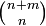
\includegraphics[scale=.6]{graphics/7f019c11129cbf4b99ccb7f7e110acb2.png}.
\item
  Compute the mean effect for each group and the difference in means
  between the groups in every case by subtracting the mean of the
  control group from the mean of the treatment group.
\item
  Report the percentage of alternative groupings for which the
  difference in means is less or equal to the actual experimentally
  observed difference in means, and the percentage for which it is
  greater.
\item
  Note that they should sum to 100\%.
\end{itemize}

Extremely dissimilar values are evidence of an effect not entirely due
to chance, but your program need not draw any conclusions.

You may assume the experimental data are known at compile time if that's
easier than loading them at run time. Test your solution on the data
given above.



\begin{wideverbatim}

(load "@lib/simul.l")  # For 'subsets'

(scl 2)

(de _stat (A)
   (let (LenA (length A)  SumA (apply + A))
      (-
         (*/ SumA LenA)
         (*/ (- SumAB SumA) (- LenAB LenA)) ) ) )

(de permutationTest (A B)
   (let
      (AB (append A B)
         SumAB (apply + AB)
         LenAB (length AB)
         Tobs (_stat A)
         Count 0 )
      (*/
         (sum
            '((Perm)
               (inc 'Count)
               (and (>= Tobs (_stat Perm)) 1) )
            (subsets (length A) AB) )
         100.0
         Count ) ) )

(setq
   *TreatmentGroup (0.85 0.88 0.75 0.66 0.25 0.29 0.83 0.39 0.97)
   *ControlGroup   (0.68 0.41 0.10 0.49 0.16 0.65 0.32 0.92 0.28 0.98) )

(let N (permutationTest *TreatmentGroup *ControlGroup)
   (prinl "under = " (round N) "\%, over = " (round (- 100.0 N)) "\%") )

Output:

under = 87.85\%, over = 12.15\%

\end{wideverbatim}

\pagebreak{}
\section*{Permutations}

Write a program which generates the all
\href{http://en.wikipedia.org/wiki/Permutation}{permutations} of
\textbf{n} different objects. (Practically numerals!)

C.f.

\begin{itemize}
\item \emph{Find the missing permutation}
\item
  \emph{Permutations/Derangements}


\begin{wideverbatim}

(load "@lib/simul.l")

(permute (1 2 3))

Output:

-> ((1 2 3) (1 3 2) (2 1 3) (2 3 1) (3 1 2) (3 2 1))

\end{wideverbatim}

\pagebreak{}
\section*{Permutations/Derangements}

A \href{http://mathworld.wolfram.com/Derangement.html}{derangement} is a
permutation of the order of distinct items in which \emph{no item
appears in its original place}.

For example, the only two derangements of the three items (0, 1, 2) are
(1, 2, 0), and (2, 0, 1).

The number of derangements of \emph{n} distinct items is known as the
subfactorial of \emph{n}, sometimes written as~!\emph{n}. There are
various ways to
\href{http://en.wikipedia.org/wiki/Derangement\#Counting\_derangements}{calculate}~!\emph{n}.

Task

The task is to:

\begin{enumerate}
\item
  Create a named function/method/subroutine/\ldots{} to generate
  derangements of the integers \emph{0..n-1}, (or \emph{1..n} if you
  prefer).
\item
  Generate \emph{and show} all the derangements of 4 integers using the
  above routine.
\item
  Create a function that calculates the subfactorial of
  \emph{n},~!\emph{n}.
\item
  Print and show a table of the \emph{counted} number of derangements of
  \emph{n} vs. the calculated~!\emph{n} for n from 0..9 inclusive.
\end{enumerate}

As an optional stretch goal:

\begin{itemize}
\item
  Calculate~!\emph{20}.
\end{itemize}

Cf.

\begin{itemize}
\item
  \emph{Anagrams/Deranged anagrams}
\item
  \emph{Best shuffle}
\end{itemize}


\end{itemize}


\begin{wideverbatim}

(load "@lib/simul.l")  # For 'permute'

(de derangements (Lst)
   (filter
      '((L) (not (find = L Lst)))
      (permute Lst) ) )

(de subfact (N)
   (if (>= 2 N)
      (if (= 1 N) 0 1)
      (*
         (dec N)
         (+ (subfact (dec N)) (subfact (- N 2))) ) ) )

Output:

: (derangements (range 1 4))
-> ((2 1 4 3) (2 3 4 1) (2 4 1 3) (3 1 4 2) (3 4 1 2) (3 4 2 1) 
(4 1 2 3)(4 3 1 2) (4 3 2 1))

: (for I (range 0 9)
   (tab (2 8 8)
      I
      (length (derangements (range 1 I)))
      (subfact I) ) )
 0       1       1
 1       0       0
 2       1       1
 3       2       2
 4       9       9
 5      44      44
 6     265     265
 7    1854    1854
 8   14833   14833
 9  133496  133496
-> NIL

: (subfact 20)
-> 895014631192902121

\end{wideverbatim}

\pagebreak{}
\section*{Pi}

Create a program to continually calculate and output the next digit of π
(pi). The program should continue forever (until it is aborted by the
user) calculating and outputting each digit in succession. The output
should be a decimal sequence beginning 3.14159265 \ldots{}

\begin{wideverbatim}

The following script uses the spigot algorithm published by Jeremy Gibbons.
Hit Ctrl-C to stop it.

#!/usr/bin/picolisp /usr/lib/picolisp/lib.l

(de piDigit ()
   (job '((Q . 1) (R . 0) (S . 1) (K . 1) (N . 3) (L . 3))
      (while (>= (- (+ R (* 4 Q)) S) (* N S))
         (mapc set '(Q R S K N L)
            (list
               (* Q K)
               (* L (+ R (* 2 Q)))
               (* S L)
               (inc K)
               (/ (+ (* Q (+ 2 (* 7 K))) (* R L)) (* S L))
               (+ 2 L) ) ) )
      (prog1 N
         (let M (- (/ (* 10 (+ R (* 3 Q))) S) (* 10 N))
            (setq Q (* 10 Q)  R (* 10 (- R (* N S)))  N M) ) ) ) )

(prin (piDigit) ".")
(loop
   (prin (piDigit))
   (flush) )

Output:

3.14159265358979323846264338327950288419716939937510582097494459 ...

\end{wideverbatim}

\pagebreak{}
\section*{Pick random element}

Demonstrate how to pick a random element from a list.

\begin{wideverbatim}

(get Lst (rand 1 (length Lst)))

\end{wideverbatim}

\pagebreak{}
\section*{Pinstripe/Display}

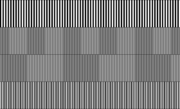
\includegraphics[scale=.6]{graphics/180px-Pinstripe-mono-unicon.png}

The task is to demonstrate the creation of a series of 1 pixel wide
vertical pinstripes across the entire width of the display. The
pinstripes should alternate one pixel white, one pixel black.

Quarter of the way down the display, we can switch to a wider 2 pixel
wide vertical pinstripe pattern, alternating two pixels white, two
pixels black. Half way down the display, we switch to 3 pixels wide, and
for the lower quarter of the display we use 4 pixels.

c.f. \emph{Colour\_pinstripe/Display}

\begin{wideverbatim}

(let Pbm  # Create PBM of 384 x 288 pixels
   (make
      (for N 4
         (let
            (C 0
               L (make
                  (do (/ 384 N)
                     (do N (link C))
                     (setq C (x| 1 C)) ) ) )
            (do 72 (link L)) ) ) )
   (out '(display)  # Pipe to ImageMagick
      (prinl "P1")
      (prinl (length (car Pbm)) " " (length Pbm))
      (mapc prinl Pbm) ) )

\end{wideverbatim}

\pagebreak{}
\section*{Pinstripe/Printer}

The task is to demonstrate the creation of a series of 1 point wide
vertical pinstripes with a sufficient number of pinstripes to span the
entire width of the printed page (except for the last pinstripe). The
pinstripes should alternate one point white, one point black. (Where the
printer does not support producing graphics in terms of points, pixels
may be substituted in this task.)

After the first inch of printing, we switch to a wider 2 point wide
vertical pinstripe pattern. alternating two points white, two points
black. We then switch to 3 points wide for the next inch, and then 4
points wide, etc. This trend continues for the entire length of the page
(or for 12 inches of run length in the case of a printer using
continuous roll stationery). After printing the test pattern the page is
ejected (or the test pattern is rolled clear of the printer enclosure,
in the case of continuous roll printers).

Note that it is an acceptable solution to use the smallest marks that
the language provides, rather than working at native printer resolution,
where this is not achievable from within the language.

Optionally, on systems where the printer resolution cannot be
determined, it is permissible to prompt the user for printer resolution,
and to calculate point size based on user input, enabling fractional
point sizes to be used.


\begin{wideverbatim}

(load "@lib/ps.l")

(call 'lpr
   (pdf "pinstripes"
      (a4)  # 595 x 842 dots
      (for X 595
         (gray (if (bit? 1 X) 0 100)
            (vline X 0 842) ) )
      (page) ) )

\end{wideverbatim}

\pagebreak{}
\section*{Play recorded sounds}

Load at least two prerecorded sounds, and demonstrate as many of
these~features as you can:

\begin{itemize}
\item
  playing them individually and simultaneously
\item
  stopping before the end of the sound
\item
  looping (preferably glitch-free)
\item
  setting the volume of each sound
\item
  stereo or 3D positional mixing
\item
  performing other actions when marked times in the sound arrive
\end{itemize}

Describe:

\begin{itemize}
\item
  The supported audio formats, briefly.
\item
  Whether it is suitable for game sound effects (low-latency start,
  resource efficiency, supports many simultaneous sounds, etc.)
\item
  Whether it is suitable for playing music (long duration ).
\end{itemize}

{[}Note: If it seems to be a good idea, this task may be revised to
specify a particular timeline rather than just `demonstrate these
features'.{]}

Where applicable, please categorize examples primarily by the audio
facility used (library/API/program/platform) rather than the language if
the language is incidental (e.g. ``Mac OS X CoreAudio'' or ``mplayer''
rather than ``C'' or ``bash'').



\begin{wideverbatim}

The obvious way is to call 'sox', the "Swiss Army knife of audio manipulation"
(man sox).

The following plays two files "a.wav" and "b.wav" simultaneously (to play them
individually, omit the "-m" flag). The first one is played with a volume of 75
percent, the second with 25 percent, starting at the 4th second, with a duration
of 6 seconds, looping 5 times.

(call 'sox
   "-m"  "-v" "0.75" "a.wav"  "-v" "0.25" "b.wav"
   "-d"
   "trim" 4 6
   "repeat" 5 )

\end{wideverbatim}

\pagebreak{}
\section*{Playing cards}

Create a data structure and the associated methods to define and
manipulate a deck of
\href{http://en.wikipedia.org/wiki/Playing-cards\#Anglo-American-French}{playing
cards}. The deck should contain 52 unique cards. The methods must
include the ability to make a new deck, shuffle (randomize) the deck,
deal from the deck, and print the current contents of a deck. Each card
must have a pip value and a suit value which constitute the unique value
of the card.

\begin{wideverbatim}

(de *Suits
   Club Diamond Heart Spade )

(de *Pips
   Ace 2 3 4 5 6 7 8 9 10 Jack Queen King )

(de mkDeck ()
   (mapcan
      '((Pip) (mapcar cons *Suits (circ Pip)))
      *Pips ) )

(de shuffle (Lst)
   (by '(NIL (rand)) sort Lst) )

\end{wideverbatim}

\pagebreak{}
\section*{Plot coordinate pairs}

Plot a function represented as `x', `y' numerical arrays.

Post link to your resulting image for input arrays (see
\emph{\textbf{Example} section for Python
language on \emph{Query Performance} page}):

\begin{wideverbatim}
x = {0, 1, 2, 3, 4, 5, 6, 7, 8, 9};
y = {2.7, 2.8, 31.4, 38.1, 58.0, 76.2, 100.5, 130.0, 149.3, 180.0};
\end{wideverbatim}

This task is intended as a subtask for \emph{Measure relative
  performance of sorting algorithms implementations}.

\vspace{3cm}

Example \emph{PicoLisp} Output:

\begin{figure}[H]
  \centering
  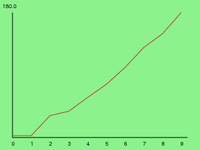
\includegraphics{graphics/200px-Plotxy-picoLisp.png}
  % \caption{Example PicoLisp Output}
  \label{fig:plotxy-picolisp}
\end{figure}


\begin{wideverbatim}

(load "@lib/ps.l")

(scl 1)

(de plot (PsFile DX DY Lst)
   (let (SX (length Lst)  SY (apply max Lst)  N 0 Val)
      (out PsFile
         (psHead (+ DX 20) (+ DY 40))
         (font (9 . "Helvetica"))
         (if (or (=0 SX) (=0 SY))
            (window 60 12 DX DY
               (font 24 ,"Not enough Data") )
            (setq Lst  # Build coordinates
               (let X -1
                  (mapcar
                     '((Y)
                        (cons
                           (*/ (inc 'X) DX SX)
                           (- DY (*/ Y DY SY)) ) )
                     Lst ) ) )
            (color 55 95 55  # Background color
               (let (X (+ DX 40) Y (+ DY 40))
                  (poly T  0 0  X 0  X Y  0 Y  0 0) ) )
            (window 20 20 DX DY  # Plot coordinates
               (poly NIL 0 0  0 DY  (- DX 20) DY)
               (color 76 24 24
                  (poly NIL (caar Lst) (cdar Lst) (cdr Lst)) ) )
            (window 4 4 60 12 (ps (format SY *Scl)))
            (for X SX
               (window (+ 6 (*/ (dec X) DX SX)) (+ 24 DY) 30 12
                  (ps (format (dec X)) 0) ) ) )
         (page) ) ) )

(plot "plot.ps" 300 200 (2.7 2.8 31.4 38.1 58.0 76.2 100.5 130.0 149.3 180.0))
(call 'display "plot.ps")

\end{wideverbatim}

\pagebreak{}
\section*{Pointers and references}

\textbf{Basic Data Operation}\\ This is a basic data operation. It
represents a fundamental action on a basic data type.

You may see other such operations in the \emph{Basic Data Operations}
category, or:

\textbf{Integer Operations} \\
\emph{Arithmetic} \textbar{} \emph{Comparison}

\textbf{Boolean Operations} \\ \emph{Bitwise} \textbar{}
\emph{Logical}

\textbf{String Operations} \\
\emph{Concatenation} \textbar{} \emph{Interpolation} \textbar{}
\emph{Matching}

\textbf{Memory Operations} \\ \textbf{Pointers \& references}
\textbar{} \emph{Addresses}

In this task, the goal is to demonstrate common operations on pointers
and references.


\begin{wideverbatim}

The internal PicoLisp machinery consists completely of pointers. Any data item
(except numbers) is a pointer that points to a cell, which in turn consists of
two pointers ("cons pair").

The pointers are not evident to the programmer. The development environment
presents them as high level structures (symbols or lists). However, the pointer
value (the address) can be obtained with the
'[http://software-lab.de/doc/refA.html#adr adr]' function.

"Dereferencing" a pointer is done with the
'[http://software-lab.de/doc/refC.html#car car]' or
'[http://software-lab.de/doc/refV.html#val val]' functions. They return the data
item at the memory location (CAR or VAL part of a cell). With
'[http://software-lab.de/doc/refS.html#set set]', a value can be stored in the
referred location.

There is no meaningful pointer arithmetics, except functions like
'[http://software-lab.de/doc/refC.html#cdr cdr]' or
'[http://software-lab.de/doc/refN.html#nth nth]', which advance the pointer to
the next (linked to) location(s).

: (setq L (1 a 2 b 3 c))         # Create a list of 6 items in 'L'
-> (1 a 2 b 3 c)

: (nth L 4)                      # Get a pointer to the 4th item
-> (b 3 c)

: (set (nth L 4) "Hello")        # Store "Hello" in that location
-> "Hello"

: L                              # Look at the modified list in 'L'
-> (1 a 2 "Hello" 3 c)

\end{wideverbatim}

\pagebreak{}
\section*{Polynomial long division}

In algebra,
\href{http://en.wikipedia.org/wiki/Polynomial\_long\_division}{polynomial
  long division} is an algorithm for dividing a polynomial by another
polynomial of the same or lower degree.

Let us suppose a polynomial is represented by a vector, \emph{x} (i.e.,
an ordered collection of
\href{http://en.wikipedia.org/wiki/Coefficient}{coefficients}) so that
the \emph{i}\textsuperscript{th} element keeps the coefficient of
\emph{x}\textsuperscript{\emph{i}}, and the multiplication by a monomial
is a \emph{shift} of the vector's elements ``towards right'' (injecting
zeros from left) followed by a multiplication of each element by the
coefficient of the monomial.

Then a pseudocode for the polynomial long division using the conventions
described above could be:

\begin{wideverbatim}
degree(P):
  return the index of the last non-zero element of P;
         if all elements are 0, return -∞

polynomial_long_division(N, D) returns (q, r):
  // N, D, q, r are vectors
  if degree(D) < 0 then error
  if degree(N) ≥ degree(D) then
    q ← 0
    while degree(N) ≥ degree(D)
      d ← D shifted right by (degree(N) - degree(D))
      q(degree(N) - degree(D)) ← N(degree(N)) / d(degree(d))
      // by construction, degree(d) = degree(N) of course
      d ← d * q(degree(N) - degree(D))
      N ← N - d
    endwhile
    r ← N
  else
    q ← 0
    r ← N
  endif
  return (q, r)
\end{wideverbatim}

\pagebreak{}

\textbf{Note}: \texttt{vector * scalar} multiplies each element of the
vector by the scalar; \texttt{vectorA - vectorB} subtracts each element
of the vectorB from the element of the vectorA with ``the same index''.
The vectors in the pseudocode are zero-based.

\begin{itemize}
\item
  Error handling (for allocations or for wrong inputs) is not mandatory.
\item
  Conventions can be different; in particular, note that if the first
  coefficient in the vector is the highest power of x for the polynomial
  represented by the vector, then the algorithm becomes simpler.
\end{itemize}

\textbf{Example for clarification} \\ This example is from Wikipedia,
but changed to show how the given pseudocode works.

\begin{wideverbatim}
      0    1    2    3
   ----------------------
N:  -42    0  -12    1        degree = 3
D:   -3    1    0    0        degree = 1

   d(N) - d(D) = 2, so let's shift D towards right by 2:

N:  -42    0  -12    1
d:    0    0   -3    1

   N(3)/d(3) = 1, so d is unchanged. Now remember that "shifting by 2"
   is like multiplying by x2, and the final multiplication
   (here by 1) is the coefficient of this monomial. Let's store this
   into q:
                               0     1     2
                              ---------------
                          q:   0     0     1

   now compute N - d, and let it be the "new" N, and let's loop

N:  -42    0   -9    0        degree = 2
D:   -3    1    0    0        degree = 1

   d(N) - d(D) = 1, right shift D by 1 and let it be d

N:  -42    0   -9    0
d:    0   -3    1    0        * -9/1 = -9

                          q:   0    -9     1

d:    0   27   -9    0        

   N ← N - d

N:  -42  -27    0    0        degree = 1
D:   -3    1    0    0        degree = 1

   looping again... d(N)-d(D)=0, so no shift is needed; we
   multiply D by -27 (= -27/1) storing the result in d, then

                          q:  -27   -9     1

   and

N:  -42  -27    0    0        -
d:   81  -27    0    0        =
N: -123    0    0    0        (last N)

    d(N) < d(D), so now r ← N, and the result is:

       0   1  2
   -------------
q:   -27  -9  1   →  x2 - 9x - 27
r:  -123   0  0   →          -123
\end{wideverbatim}



\begin{wideverbatim}

(de degree (P)
   (let I NIL
      (for (N . C) P
         (or (=0 C) (setq I N)) )
      (dec I) ) )

(de divPoly (N D)
   (if (lt0 (degree D))
      (quit "Div/0" D)
      (let (Q NIL Diff)
         (while (ge0 (setq Diff (- (degree N) (degree D))))
            (setq Q (need (- -1 Diff) Q 0))
            (let E D
               (do Diff (push 'E 0))
               (let F (/ (get N (inc (degree N))) (get E (inc (degree E))))
                  (set (nth Q (inc Diff)) F)
                  (setq N (mapcar '((N E) (- N (* E F))) N E)) ) ) )
         (list Q N) ) ) )

Output:

: (divPoly (-42 0 -12 1) (-3 1 0 0))
-> ((-27 -9 1) (-123 0 0 0))

\end{wideverbatim}

\pagebreak{}
\section*{Polymorphic copy}


An object is \emph{polymorphic} when its specific
type may vary. The types a specific value may take, is called
\emph{class}.

It is trivial to copy an object if its type is known:

\begin{verbatim}
  int x;
  int y = x;
\end{verbatim}

Here x is not polymorphic, so y is declared of same type (\emph{int}) as
x. But if the specific type of x were unknown, then y could not be
declared of any specific type.

The task: let a polymorphic object contain an instance of some specific
type S derived from a type T. The type T is known. The type S is
possibly unknown until \emph{run time}. The objective
is to create an exact copy of such polymorphic object (not to create a
\emph{reference}, nor a pointer to). Let further the
type T have a method overridden by S. This method is to be called on the
copy to demonstrate that the specific type of the copy is indeed S.

\begin{wideverbatim}

Any object can be copied by transferring the value and the property list. If we
create an object 'A':

: (setq A (new '(+Cls1 +Cls2) 'attr1 123  'attr2 "def"  'attr3 (4 2 0)  'attr4 T
-> \$385603635

: (show A)
\$385603635 (+Cls1 +Cls2)
   attr4
   attr3 (4 2 0)
   attr2 "def"
   attr1 123
-> \$385603635

Then we can easily copy it to a new object 'B':

(putl (setq B (new (val A))) (getl A))

Inspecting 'B':

: (show B)
\$385346595 (+Cls1 +Cls2)
   attr1 123
   attr2 "def"
   attr3 (4 2 0)
   attr4
-> \$385346595

\end{wideverbatim}

\pagebreak{}
\section*{Polymorphism}

Create two classes Point(x,y) and Circle(x,y,r) with a polymorphic
function print, accessors for (x,y,r), copy constructor, assignment and
destructor and every possible default constructors

\begin{wideverbatim}

(class +Point)
# x y

(dm T (X Y)
   (=: x (or X 0))
   (=: y (or Y 0)) )

(dm print> ()
   (prinl "Point " (: x) "," (: y)) )

(class +Circle +Point)
# r

(dm T (X Y R)
   (super X Y)
   (=: r (or R 0)) )

(dm print> ()
   (prinl "Circle " (: x) "," (: y) "," (: r)) )


(setq
   P (new '(+Point) 3 4)
   C (new '(+Circle) 10 10 5) )

(print> P)
(print> C)

Output:

Point 3,4
Circle 10,10,5

\end{wideverbatim}

\pagebreak{}
\section*{Power set}

A \emph{set} is a collection (container) of certain values,
without any particular order, and no repeated values. It corresponds
with a finite set in mathematics. A set can be implemented as an
associative array (partial mapping) in which the value of each key-value
pair is ignored.

Given a set S, the \href{http://en.wikipedia.org/wiki/Power\_set}{power
set} (or powerset) of S, written P(S), or 2\textsuperscript{S}, is the
set of all subsets of S.

\textbf{Task~:} By using a library or build-in set type, or defining a
set type with necessary operations, write a function with a set S as
input that yields a power set 2\textsuperscript{S} of S.

For example, the power set of \{1,2,3,4\} is \{\{\}, \{1\}, \{2\},
\{1,2\}, \{3\}, \{1,3\}, \{2,3\}, \{1,2,3\}, \{4\}, \{1,4\}, \{2,4\},
\{1,2,4\}, \{3,4\}, \{1,3,4\}, \{2,3,4\}, \{1,2,3,4\}\}.


\begin{wideverbatim}

(de powerset (Lst)
   (ifn Lst
      (cons)
      (let L (powerset (cdr Lst))
         (conc
            (mapcar '((X) (cons (car Lst) X)) L)
            L ) ) ) )

\end{wideverbatim}

\pagebreak{}
\section*{Pragmatic directives}

Pragmatic directives cause the language to operate in a specific manner,
allowing support for operational variances within the program code
(possibly by the loading of specific or alternative modules).

The task is to list any pragmatic directives supported by the language,
demostrate how to activate and deactivate the pragmatic directives and
to describe or demonstate the scope of effect that the pragmatic
directives have within a program.

\begin{wideverbatim}

PicoLisp makes no formal difference between any normal and "specific" operation
of the language. Any possible desired effect can be achieved by calling a
function or setting a variable. For example, function calls can be traced with
the '[http://software-lab.de/doc/refT.html#trace trace]' function.

\end{wideverbatim}

\pagebreak{}
\section*{Price Fraction}

A friend of mine runs a pharmacy. He has a specialised function in his
Dispensary application which receives a decimal value of currency and
replaces it to a standard value. This value is regulated by a government
department.

Task: Given a floating point value between 0.00 and 1.00, rescale
according to the following table:

\begin{verbatim}
>=  0.00  <  0.06  :=  0.10
>=  0.06  <  0.11  :=  0.18
>=  0.11  <  0.16  :=  0.26
>=  0.16  <  0.21  :=  0.32
>=  0.21  <  0.26  :=  0.38
>=  0.26  <  0.31  :=  0.44
>=  0.31  <  0.36  :=  0.50
>=  0.36  <  0.41  :=  0.54
>=  0.41  <  0.46  :=  0.58
>=  0.46  <  0.51  :=  0.62
>=  0.51  <  0.56  :=  0.66
>=  0.56  <  0.61  :=  0.70
>=  0.61  <  0.66  :=  0.74
>=  0.66  <  0.71  :=  0.78
>=  0.71  <  0.76  :=  0.82
>=  0.76  <  0.81  :=  0.86
>=  0.81  <  0.86  :=  0.90
>=  0.86  <  0.91  :=  0.94
>=  0.91  <  0.96  :=  0.98
>=  0.96  <  1.01  :=  1.00
\end{verbatim}

\begin{wideverbatim}

(scl 2)

(de price (Pr)
   (format
      (cdr
         (rank Pr
            (quote
               (0.00 . 0.10)
               (0.06 . 0.18)
               (0.11 . 0.26)
               (0.16 . 0.32)
               (0.21 . 0.38)
               (0.26 . 0.44)
               (0.31 . 0.50)
               (0.36 . 0.54)
               (0.41 . 0.58)
               (0.46 . 0.62)
               (0.51 . 0.66)
               (0.56 . 0.70)
               (0.61 . 0.74)
               (0.66 . 0.78)
               (0.71 . 0.82)
               (0.76 . 0.86)
               (0.81 . 0.90)
               (0.86 . 0.94)
               (0.91 . 0.98)
               (0.96 . 1.00) ) ) )
      *Scl ) )

(for N (0.3793 0.4425 0.0746 0.6918 0.2993 0.5486 0.7848 0.9383 0.2292)
   (prinl (price N)) )

Output:

0.54
0.58
0.18
0.78
0.44
0.66
0.86
0.98
0.38

\end{wideverbatim}

\pagebreak{}
\section*{Primality by trial division}

Write a boolean function that tells whether a given integer is prime.
Remember that 1 and all non-positive numbers are not prime.

Use trial division. Even numbers over two may be eliminated right away.
A loop from 3 to √n will suffice, but other loops are allowed.

\begin{itemize}
\item Related task: \emph{Sieve of Eratosthenes}, \emph{Prime
    decomposition}.
\end{itemize}

\begin{wideverbatim}

(de prime? (N)
   (or
      (= N 2)
      (and
         (> N 1)
         (bit? 1 N)
         (for (D 3  T  (+ D 2))
            (T (> D (sqrt N)) T)
            (T (=0 (\% N D)) NIL) ) ) ) )

\end{wideverbatim}

\pagebreak{}
\section*{Prime decomposition}

The prime decomposition of a number is defined as a list of prime
numbers which when all multiplied together, are equal to that number.
Example: 12 = 2 × 2 × 3, so its prime decomposition is \{2, 2, 3\}

Write a function which returns an \emph{array} or \emph{collection}
which contains the prime decomposition of a given number, n, greater
than 1. If your language does not have an isPrime-like function
available, you may assume that you have a function which determines
whether a number is prime (note its name before your code).

If you would like to test code from this task, you may use code from
\emph{trial division} or the \emph{Sieve of Eratosthenes}.

Note: The program must not be limited by the word size of your computer
or some other artificial limit; it should work for any number regardless
of size (ignoring the physical limits of RAM etc).

\begin{wideverbatim}

The following solution generates a sequence of "trial divisors" (2 3 5 7 11 13
17 19 23 29 31 37 ..), as described by Donald E. Knuth, "The Art of Computer
Programming", Vol.2, p.365.

(de factor (N)
   (make
      (let (D 2  L (1 2 2 . (4 2 4 2 4 6 2 6 .))  M (sqrt N))
         (while (>= M D)
            (if (=0 (\% N D))
               (setq M (sqrt (setq N (/ N (link D)))))
               (inc 'D (pop 'L)) ) )
         (link N) ) ) )

(factor 1361129467683753853853498429727072845823)

Output:

-> (3 11 31 131 2731 8191 409891 7623851 145295143558111)

\end{wideverbatim}

\pagebreak{}
\section*{Priority queue}

A \href{http://en.wikipedia.org/wiki/Priority\_queue}{priority queue} is
somewhat similar to a \emph{queue}, with an important
distinction: each item is added to a priority queue with a priority
level, and will be later removed from the queue with the highest
priority element first. That is, the items are (conceptually) stored in
the queue in priority order instead of in insertion order.

\textbf{Task:} Create a priority queue. The queue must support at least
two operations:

\begin{enumerate}
\item
  Insertion. An element is added to the queue with a priority (a numeric
  value).
\item
  Top item removal. Deletes the element or one of the elements with the
  current top priority and return it.
\end{enumerate}

Optionally, other operations may be defined, such as peeking (find what
current top priority/top element is), merging (combining two priority
queues into one), etc.

To test your implementation, insert a number of elements into the queue,
each with some random priority. Then dequeue them sequentially; now the
elements should be sorted by priority. You can use the following
task/priority items as input data:

\begin{verbatim}
Priority    Task
  3        Clear drains
  4        Feed cat
  5        Make tea
  1        Solve RC tasks
  2        Tax return
\end{verbatim}

The implementation should try to be efficient. A typical implementation
has O(log n) insertion and extraction time, where n is the number of
items in the queue. You may choose to impose certain limits such as
small range of allowed priority levels, limited capacity, etc. If so,
discuss the reasons behind it.



\begin{wideverbatim}

The following implementation imposes no limits. It uses a
[http://software-lab.de/doc/refI.html#idx binary tree] for storage. The priority
levels may be numeric, or of any other type.

# Insert item into priority queue
(de insertPQ (Queue Prio Item)
   (idx Queue (cons Prio Item) T) )

# Remove and return top item from priority queue
(de removePQ (Queue)
   (cdar (idx Queue (peekPQ Queue) NIL)) )

# Find top element in priority queue
(de peekPQ (Queue)
   (let V (val Queue)
      (while (cadr V)
         (setq V @) )
      (car V) ) )

# Merge second queue into first
(de mergePQ (Queue1 Queue2)
   (balance Queue1 (sort (conc (idx Queue1) (idx Queue2)))) )

Test:

# Two priority queues
(off Pq1 Pq2)

# Insert into first queue
(insertPQ 'Pq1 3 '(Clear drains))
(insertPQ 'Pq1 4 '(Feed cat))

# Insert into second queue
(insertPQ 'Pq2 5 '(Make tea))
(insertPQ 'Pq2 1 '(Solve RC tasks))
(insertPQ 'Pq2 2 '(Tax return))

# Merge second into first queue
(mergePQ 'Pq1 'Pq2)

# Remove and print all items from first queue
(while Pq1
   (println (removePQ 'Pq1)) )

Output:

(Solve RC tasks)
(Tax return)
(Clear drains)
(Feed cat)
(Make tea)

\end{wideverbatim}

\pagebreak{}
\section*{Probabilistic choice}

Given a mapping between items and their required probability of
occurrence, generate a million items \emph{randomly} subject to the
given probabilities and compare the target probability of occurrence
versus the generated values.

The total of all the probabilities should equal one. (Because floating
point arithmetic is involved this is subject to rounding errors).

Use the following mapping to test your programs:

\begin{wideverbatim}
aleph   1/5.0
beth    1/6.0
gimel   1/7.0
daleth  1/8.0
he      1/9.0
waw     1/10.0
zayin   1/11.0
heth    1759/27720 # adjusted so that probabilities add to 1
\end{wideverbatim}


\begin{wideverbatim}

(let (Count 1000000  Denom 27720  N Denom)
   (let Probs
      (mapcar
         '((I S)
            (prog1 (cons N (*/ Count I) 0 S)
               (dec 'N (/ Denom I)) ) )
         (range 5 12)
         '(aleph beth gimel daleth he waw zayin heth) )
      (do Count
         (inc (cddr (rank (rand 1 Denom) Probs T))) )
      (let Fmt (-6 12 12)
         (tab Fmt NIL "Probability" "Result")
         (for X Probs
            (tab Fmt
               (cdddr X)
               (format (cadr X) 6)
               (format (caddr X) 6) ) ) ) ) )

Output:

       Probability      Result
aleph     0.200000    0.199760
beth      0.166667    0.166878
gimel     0.142857    0.142977
daleth    0.125000    0.124983
he        0.111111    0.111200
waw       0.100000    0.100173
zayin     0.090909    0.090591
heth      0.083333    0.063438

\end{wideverbatim}

\pagebreak{}
\section*{Program termination}

Show the syntax for a complete stoppage of a program inside a
\emph{conditional}. This includes all \emph{threads}/\emph{processes}
which are part of your program.

Explain the cleanup (or lack thereof) caused by the termination
(allocated memory, database connections, open files, object
finalizers/destructors, run-on-exit hooks, etc.). Unless otherwise
described, no special cleanup outside that provided by the operating
system is provided.

\begin{wideverbatim}

Calling 'bye', optionally with a numeric code, terminates the program.

This will execute all pending 'finally' expressions, close all open files and/
or pipes, flush standard output, and execute all expressions in the global
variable '*Bye' before exiting.

(push '*Bye '(prinl "Goodbye world!"))
(bye)

Output:

Goodbye world!
\$

\end{wideverbatim}

\pagebreak{}
\section*{Pythagorean triples}

A \href{http://en.wikipedia.org/wiki/Pythagorean\_triple}{Pythagorean
triple} is defined as three positive integers
(\emph{a},\emph{b},\emph{c}) where \emph{a} \textless{} \emph{b}
\textless{} \emph{c}, and \emph{a}\textsuperscript{2} +
\emph{b}\textsuperscript{2} = \emph{c}\textsuperscript{2}. They are
called primitive triples if \emph{a},\emph{b},\emph{c} are coprime, that
is, if their pairwise greatest common divisors gcd(\emph{a},\emph{b}) =
gcd(\emph{a},\emph{c}) = gcd(\emph{b},\emph{c}) = 1. Because of their
relationship through the Pythagorean theorem, a, b, and c are coprime if
a and b are coprime (gcd(\emph{a},\emph{b}) = 1). Each triple forms the
length of the sides of a right triangle, whose perimeter is \emph{P} =
\emph{a} + \emph{b} + \emph{c}.

\textbf{Task}

The task is to determine how many Pythagorean triples there are with a
perimeter no larger than 100 and the number of these that are primitive.

\textbf{Extra credit:} Deal with large values. Can your program handle a
max perimeter of 1,000,000? What about 10,000,000? 100,000,000?

Note: the extra credit is not for you to demonstrate how fast your
language is compared to others; you need a proper algorithm to solve
them in a timely manner.

\begin{description}
\item[Cf]
\end{description}

\begin{itemize}
\item
  \emph{List comprehensions}
\end{itemize}



\begin{wideverbatim}

(for (Max 10  (>= 100000000 Max)  (* Max 10))
   (let (Total 0  Prim 0  In (3 4 5))
      (recur (In)
         (let P (apply + In)
            (when (>= Max P)
               (inc 'Prim)
               (inc 'Total (/ Max P))
               (for Row
                  (quote
                     (( 1 -2 2) ( 2 -1 2) ( 2 -2 3))
                     (( 1  2 2) ( 2  1 2) ( 2  2 3))
                     ((-1  2 2) (-2  1 2) (-2  2 3)) )
                  (recurse
                     (mapcar '((U) (sum * U In)) Row) ) ) ) ) )
      (prinl "Up to " Max ": " Total " triples, " Prim " primitives.") ) )

Output:

Up to 10: 0 triples, 0 primitives.
Up to 100: 17 triples, 7 primitives.
Up to 1000: 325 triples, 70 primitives.
Up to 10000: 4858 triples, 703 primitives.
Up to 100000: 64741 triples, 7026 primitives.
Up to 1000000: 808950 triples, 70229 primitives.
Up to 10000000: 9706567 triples, 702309 primitives.
Up to 100000000: 113236940 triples, 7023027 primitives.

\end{wideverbatim}



% %%%%%%%%%%%%%%%%%%%%%%%% referenc.tex %%%%%%%%%%%%%%%%%%%%%%%%%%%%%%
% sample references
% %
% Use this file as a template for your own input.
%
%%%%%%%%%%%%%%%%%%%%%%%% Springer-Verlag %%%%%%%%%%%%%%%%%%%%%%%%%%
%
% BibTeX users please use
% \bibliographystyle{}
% \bibliography{}
%
\biblstarthook{In view of the parallel print and (chapter-wise) online publication of your book at \url{www.springerlink.com} it has been decided that -- as a genreral rule --  references should be sorted chapter-wise and placed at the end of the individual chapters. However, upon agreement with your contact at Springer you may list your references in a single seperate chapter at the end of your book. Deactivate the class option \texttt{sectrefs} and the \texttt{thebibliography} environment will be put out as a chapter of its own.\\\indent
References may be \textit{cited} in the text either by number (preferred) or by author/year.\footnote{Make sure that all references from the list are cited in the text. Those not cited should be moved to a separate \textit{Further Reading} section or chapter.} The reference list should ideally be \textit{sorted} in alphabetical order -- even if reference numbers are used for the their citation in the text. If there are several works by the same author, the following order should be used: 
\begin{enumerate}
\item all works by the author alone, ordered chronologically by year of publication
\item all works by the author with a coauthor, ordered alphabetically by coauthor
\item all works by the author with several coauthors, ordered chronologically by year of publication.
\end{enumerate}
The \textit{styling} of references\footnote{Always use the standard abbreviation of a journal's name according to the ISSN \textit{List of Title Word Abbreviations}, see \url{http://www.issn.org/en/node/344}} depends on the subject of your book:
\begin{itemize}
\item The \textit{two} recommended styles for references in books on \textit{mathematical, physical, statistical and computer sciences} are depicted in ~\cite{science-contrib, science-online, science-mono, science-journal, science-DOI} and ~\cite{phys-online, phys-mono, phys-journal, phys-DOI, phys-contrib}.
\item Examples of the most commonly used reference style in books on \textit{Psychology, Social Sciences} are~\cite{psysoc-mono, psysoc-online,psysoc-journal, psysoc-contrib, psysoc-DOI}.
\item Examples for references in books on \textit{Humanities, Linguistics, Philosophy} are~\cite{humlinphil-journal, humlinphil-contrib, humlinphil-mono, humlinphil-online, humlinphil-DOI}.
\item Examples of the basic Springer style used in publications on a wide range of subjects such as \textit{Computer Science, Economics, Engineering, Geosciences, Life Sciences, Medicine, Biomedicine} are ~\cite{basic-contrib, basic-online, basic-journal, basic-DOI, basic-mono}. 
\end{itemize}
}

\begin{thebibliography}{99.}%
% and use \bibitem to create references.
%
% Use the following syntax and markup for your references if 
% the subject of your book is from the field 
% "Mathematics, Physics, Statistics, Computer Science"
%
% Contribution 
\bibitem{science-contrib} Broy, M.: Software engineering --- from auxiliary to key technologies. In: Broy, M., Dener, E. (eds.) Software Pioneers, pp. 10-13. Springer, Heidelberg (2002)
%
% Online Document
\bibitem{science-online} Dod, J.: Effective substances. In: The Dictionary of Substances and Their Effects. Royal Society of Chemistry (1999) Available via DIALOG. \\
\url{http://www.rsc.org/dose/title of subordinate document. Cited 15 Jan 1999}
%
% Monograph
\bibitem{science-mono} Geddes, K.O., Czapor, S.R., Labahn, G.: Algorithms for Computer Algebra. Kluwer, Boston (1992) 
%
% Journal article
\bibitem{science-journal} Hamburger, C.: Quasimonotonicity, regularity and duality for nonlinear systems of partial differential equations. Ann. Mat. Pura. Appl. \textbf{169}, 321--354 (1995)
%
% Journal article by DOI
\bibitem{science-DOI} Slifka, M.K., Whitton, J.L.: Clinical implications of dysregulated cytokine production. J. Mol. Med. (2000) doi: 10.1007/s001090000086 
%
\bigskip

% Use the following (APS) syntax and markup for your references if 
% the subject of your book is from the field 
% "Mathematics, Physics, Statistics, Computer Science"
%
% Online Document
\bibitem{phys-online} J. Dod, in \textit{The Dictionary of Substances and Their Effects}, Royal Society of Chemistry. (Available via DIALOG, 1999), 
\url{http://www.rsc.org/dose/title of subordinate document. Cited 15 Jan 1999}
%
% Monograph
\bibitem{phys-mono} H. Ibach, H. L\"uth, \textit{Solid-State Physics}, 2nd edn. (Springer, New York, 1996), pp. 45-56 
%
% Journal article
\bibitem{phys-journal} S. Preuss, A. Demchuk Jr., M. Stuke, Appl. Phys. A \textbf{61}
%
% Journal article by DOI
\bibitem{phys-DOI} M.K. Slifka, J.L. Whitton, J. Mol. Med., doi: 10.1007/s001090000086
%
% Contribution 
\bibitem{phys-contrib} S.E. Smith, in \textit{Neuromuscular Junction}, ed. by E. Zaimis. Handbook of Experimental Pharmacology, vol 42 (Springer, Heidelberg, 1976), p. 593
%
\bigskip
%
% Use the following syntax and markup for your references if 
% the subject of your book is from the field 
% "Psychology, Social Sciences"
%
%
% Monograph
\bibitem{psysoc-mono} Calfee, R.~C., \& Valencia, R.~R. (1991). \textit{APA guide to preparing manuscripts for journal publication.} Washington, DC: American Psychological Association.
%
% Online Document
\bibitem{psysoc-online} Dod, J. (1999). Effective substances. In: The dictionary of substances and their effects. Royal Society of Chemistry. Available via DIALOG. \\
\url{http://www.rsc.org/dose/Effective substances.} Cited 15 Jan 1999.
%
% Journal article
\bibitem{psysoc-journal} Harris, M., Karper, E., Stacks, G., Hoffman, D., DeNiro, R., Cruz, P., et al. (2001). Writing labs and the Hollywood connection. \textit{J Film} Writing, 44(3), 213--245.
%
% Contribution 
\bibitem{psysoc-contrib} O'Neil, J.~M., \& Egan, J. (1992). Men's and women's gender role journeys: Metaphor for healing, transition, and transformation. In B.~R. Wainrig (Ed.), \textit{Gender issues across the life cycle} (pp. 107--123). New York: Springer.
%
% Journal article by DOI
\bibitem{psysoc-DOI}Kreger, M., Brindis, C.D., Manuel, D.M., Sassoubre, L. (2007). Lessons learned in systems change initiatives: benchmarks and indicators. \textit{American Journal of Community Psychology}, doi: 10.1007/s10464-007-9108-14.
%
%
% Use the following syntax and markup for your references if 
% the subject of your book is from the field 
% "Humanities, Linguistics, Philosophy"
%
\bigskip
%
% Journal article
\bibitem{humlinphil-journal} Alber John, Daniel C. O'Connell, and Sabine Kowal. 2002. Personal perspective in TV interviews. \textit{Pragmatics} 12:257--271
%
% Contribution 
\bibitem{humlinphil-contrib} Cameron, Deborah. 1997. Theoretical debates in feminist linguistics: Questions of sex and gender. In \textit{Gender and discourse}, ed. Ruth Wodak, 99--119. London: Sage Publications.
%
% Monograph
\bibitem{humlinphil-mono} Cameron, Deborah. 1985. \textit{Feminism and linguistic theory.} New York: St. Martin's Press.
%
% Online Document
\bibitem{humlinphil-online} Dod, Jake. 1999. Effective substances. In: The dictionary of substances and their effects. Royal Society of Chemistry. Available via DIALOG. \\
http://www.rsc.org/dose/title of subordinate document. Cited 15 Jan 1999
%
% Journal article by DOI
\bibitem{humlinphil-DOI} Suleiman, Camelia, Daniel C. O�Connell, and Sabine Kowal. 2002. `If you and I, if we, in this later day, lose that sacred fire...�': Perspective in political interviews. \textit{Journal of Psycholinguistic Research}. doi: 10.1023/A:1015592129296.
%
%
%
\bigskip
%
%
% Use the following syntax and markup for your references if 
% the subject of your book is from the field 
% "Computer Science, Economics, Engineering, Geosciences, Life Sciences"
%
%
% Contribution 
\bibitem{basic-contrib} Brown B, Aaron M (2001) The politics of nature. In: Smith J (ed) The rise of modern genomics, 3rd edn. Wiley, New York 
%
% Online Document
\bibitem{basic-online} Dod J (1999) Effective Substances. In: The dictionary of substances and their effects. Royal Society of Chemistry. Available via DIALOG. \\
\url{http://www.rsc.org/dose/title of subordinate document. Cited 15 Jan 1999}
%
% Journal article by DOI
\bibitem{basic-DOI} Slifka MK, Whitton JL (2000) Clinical implications of dysregulated cytokine production. J Mol Med, doi: 10.1007/s001090000086
%
% Journal article
\bibitem{basic-journal} Smith J, Jones M Jr, Houghton L et al (1999) Future of health insurance. N Engl J Med 965:325--329
%
% Monograph
\bibitem{basic-mono} South J, Blass B (2001) The future of modern genomics. Blackwell, London 
%
\end{thebibliography}

